\chapter{Volumetric Properties of Pure jSubstances}\label{Chapter:VolumetricPropertiesPureSubstances}

   \begin{LearningObjectivesBlock}{Learning Objectives}
      Upon completion of this chapter, you will be able to
        \begin{enumerate}
           \item Demonstrate understanding of key concepts of entropy and the second law of thermodynamics;
           \item Apply first and second laws of thermodynamics to assess of heat transfer and process reversibility;
           \item Know that Clausius inequality is an alternative statement of the second law;
           \item Demonstrate how to apply the entropy balance in a thermodynamic system;
           \item Recognise processes that generate entropy.
        \end{enumerate}
\medskip
     Recommended reading: Chapters 3 of \citet{SmithVanNess_Book}, 6 of \citet{Sandler_Book}, 2 of \citet{Borgnakke_Book} or 4 of \citet{Atkins_Book}.
   \end{LearningObjectivesBlock}

  
%%%
%%% SECTION
%%%
   \section{Introduction}\label{Chapter:VolumetricPropertiesPureSubstances:Section:Intro}
   Definitions and assumptions for ideal gas behaviour were introduced in Section~\ref{Chapter:Intro_Property_of_Gases:Section:IdealGases} along with the corresponding equation of state (Eqn.~\ref{Chapter:Intro_Property_of_Gases:Eqn:IdealEOS}). A fluid behaves as an ideal gas at low to moderate pressure (often below atmospheric pressure) and at high temperatures. Under different conditions, fluids may not behave as ideal gases and therefore other equations of state (not just for gases) were designed to describe the {\it PVT} behaviour of fluids.

Phase transition of pure substances is one of the main topics in industrial chemical engineering as it is of paramount importance to calculate fluid properties for the design of equipment and processes. Therefore, the main aim of this chapter is to introduce the concept of phase diagram of pure substances and its mathematical representation as equations of state. 

  
%%%
%%% SECTION
%%%
   \section{Phase Diagrams of Pure Substances}\label{Chapter:VolumetricPropertiesPureSubstances:Section:PhaseDiagrams}\index{Phase diagram}\index{Triple point}\index{Supercritical state}

Pure substances/fluids can be defined as materials of homogeneous and constant composition. For example, systems containing water-ice, water-steam or water-ice-steam are considered pure fluids (or substances) at different phases, whereas (a) air-water, (b) air-steam and (c) gaseous mixture containing N$_{2}$, H$_{2}$, O$_{2}$ and NO$_{2}$ are considered as either homogeneous (b-c) or heterogeneous (a) mixtures.

A pure substance can exist and coexist in different phases\footnote{Phase of a substance can be defined as the form of matter that is uniform in chemical composition and physical state.}  (\ie solid, liquid and vapour -- S, L and V). Phase behaviour of substances is often represented by {\it PVT}\footnote{{\it PVT} stands for pressure, specific (or molar) volume and temperature.} phase diagrams that describe phase transitions (\ie spontaneous conversion -- or mass/heat transfer of one phase to another) and coordinates. A 3D {\it PVT} diagram of an arbitrary substance is shown in Figure~\ref{Chapter:VolumetricPropertiesPureSubstances:Fig:PVT_Surfaces}a, where solid, liquid and vapour phases are represented by continuous volumes and, the regions between these volumes are representations of phase equilibrium, \ie regions where phases coexist in thermodynamic equilibrium.

   %%% FIGURE
           \begin{figure}[h]
              \begin{center}
                 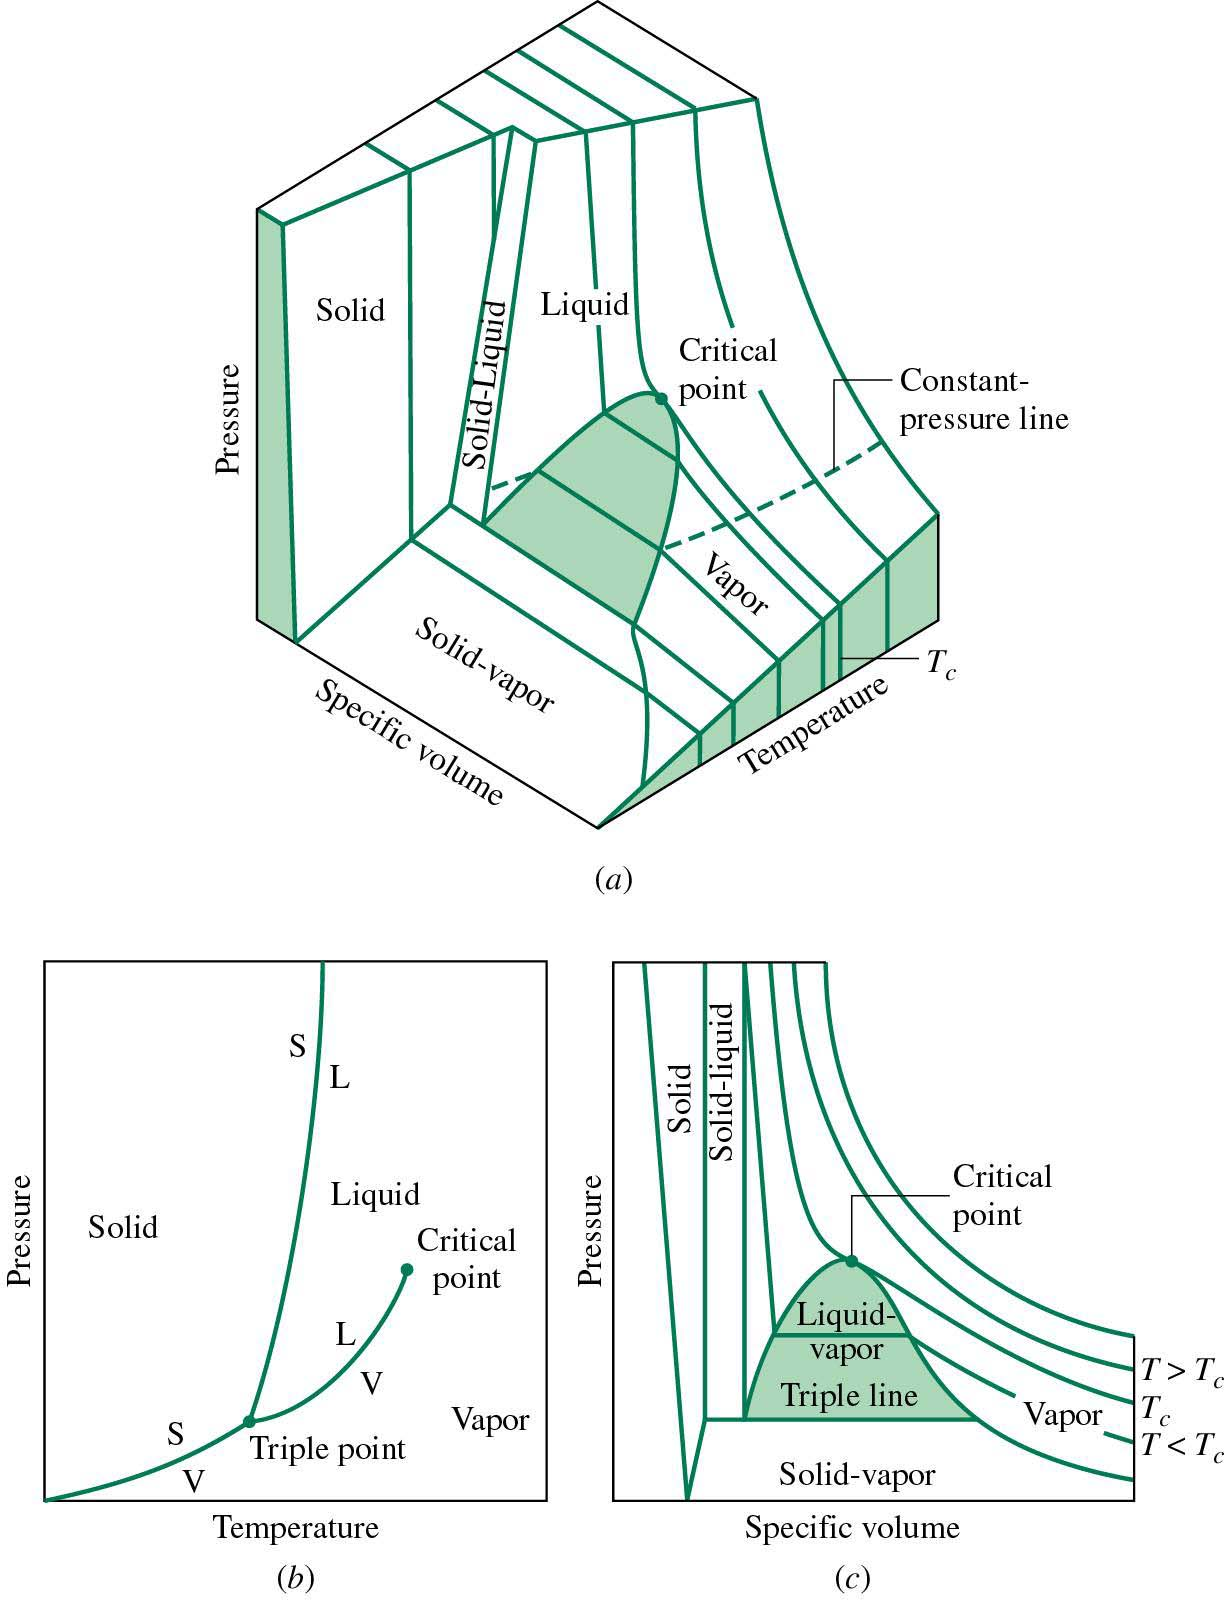
\includegraphics[width=10.cm,clip]{./Figs/PVT_Surface.jpg}
                 \caption{$PVT$ volume (top) and projections onto (b) $PT$ and (c) $PV$ diagrams for a pure substance \citep[Extracted from][]{Borgnakke_Book}.}\label{Chapter:VolumetricPropertiesPureSubstances:Fig:PVT_Surfaces}
              \end{center}
           \end{figure}    

Such 3D representation helps determining (qualitatively) phases (S, L and V) at prescribed coordinates (temperature, specific/molar volume and pressure) of fluids. However, it is not convenient dealing with 3D plots and, most of the time, we may want to extract quantitative values of fluids (Chapter~\ref{Chapter:ThermodynamicPropertiesPureFluids}). A better approach is to project 3D plots into surfaces, \ie through $PT$, $PV$ and $VT$ phase diagrams as shown in Figs.~\ref{Chapter:VolumetricPropertiesPureSubstances:Fig:PVT_Surfaces}b and \ref{Chapter:VolumetricPropertiesPureSubstances:Fig:PVT_Surfaces}c.

$PV$ diagram (Fig.~\ref{Chapter:VolumetricPropertiesPureSubstances:Fig:PV-PT_Diagrams}a) is a representation of the PVT volume, Fig.~\ref{Chapter:VolumetricPropertiesPureSubstances:Fig:PVT_Surfaces}a, where surfaces (\ie areas) represent both single phases and phases in equilibrium, and lines represent transition between phases. Here, there are three properties that we need to define:
           \begin{enumerate}[a)]
              \item Critical point (or state): coordinates in which two phases of a fluid become indistinguishable. Beyond this coordinate, a fluid is neither completely liquid nor completely gaseous, \ie exhibits properties of both the liquid phase and the gas phase and is referred to as a {\it supercritical fluid}. All fluids have distinct critical coordinates, known as {\it critical pressure} $\left(\text{P}_{c}\right)$, {\it critical temperature} $\left(\text{T}_{c}\right)$ and {\it critical volume} $\left(\text{V}_{c}\right)$. Interesting videos about critical state can be seen in 
                  \begin{center}
                     \href{https://www.youtube.com/watch?v=bJjcTpRzXpM}{https://www.youtube.com/watch?v=bJjcTpRzXpM} and \\
                     \href{https://www.youtube.com/watch?v=RmaJVxafesU}{https://www.youtube.com/watch?v=RmaJVxafesU}.
                  \end{center}
              \item Saturation lines (blue lines in Fig.~\ref{Chapter:VolumetricPropertiesPureSubstances:Fig:PV-PT_Diagrams}a) are coordinates in which phase transition starts to occur.
              \item Isotherms: Lines of constant temperature.
           \end{enumerate}

   %%% FIGURE
           \begin{figure}[h]
              \vbox{
                    \hbox{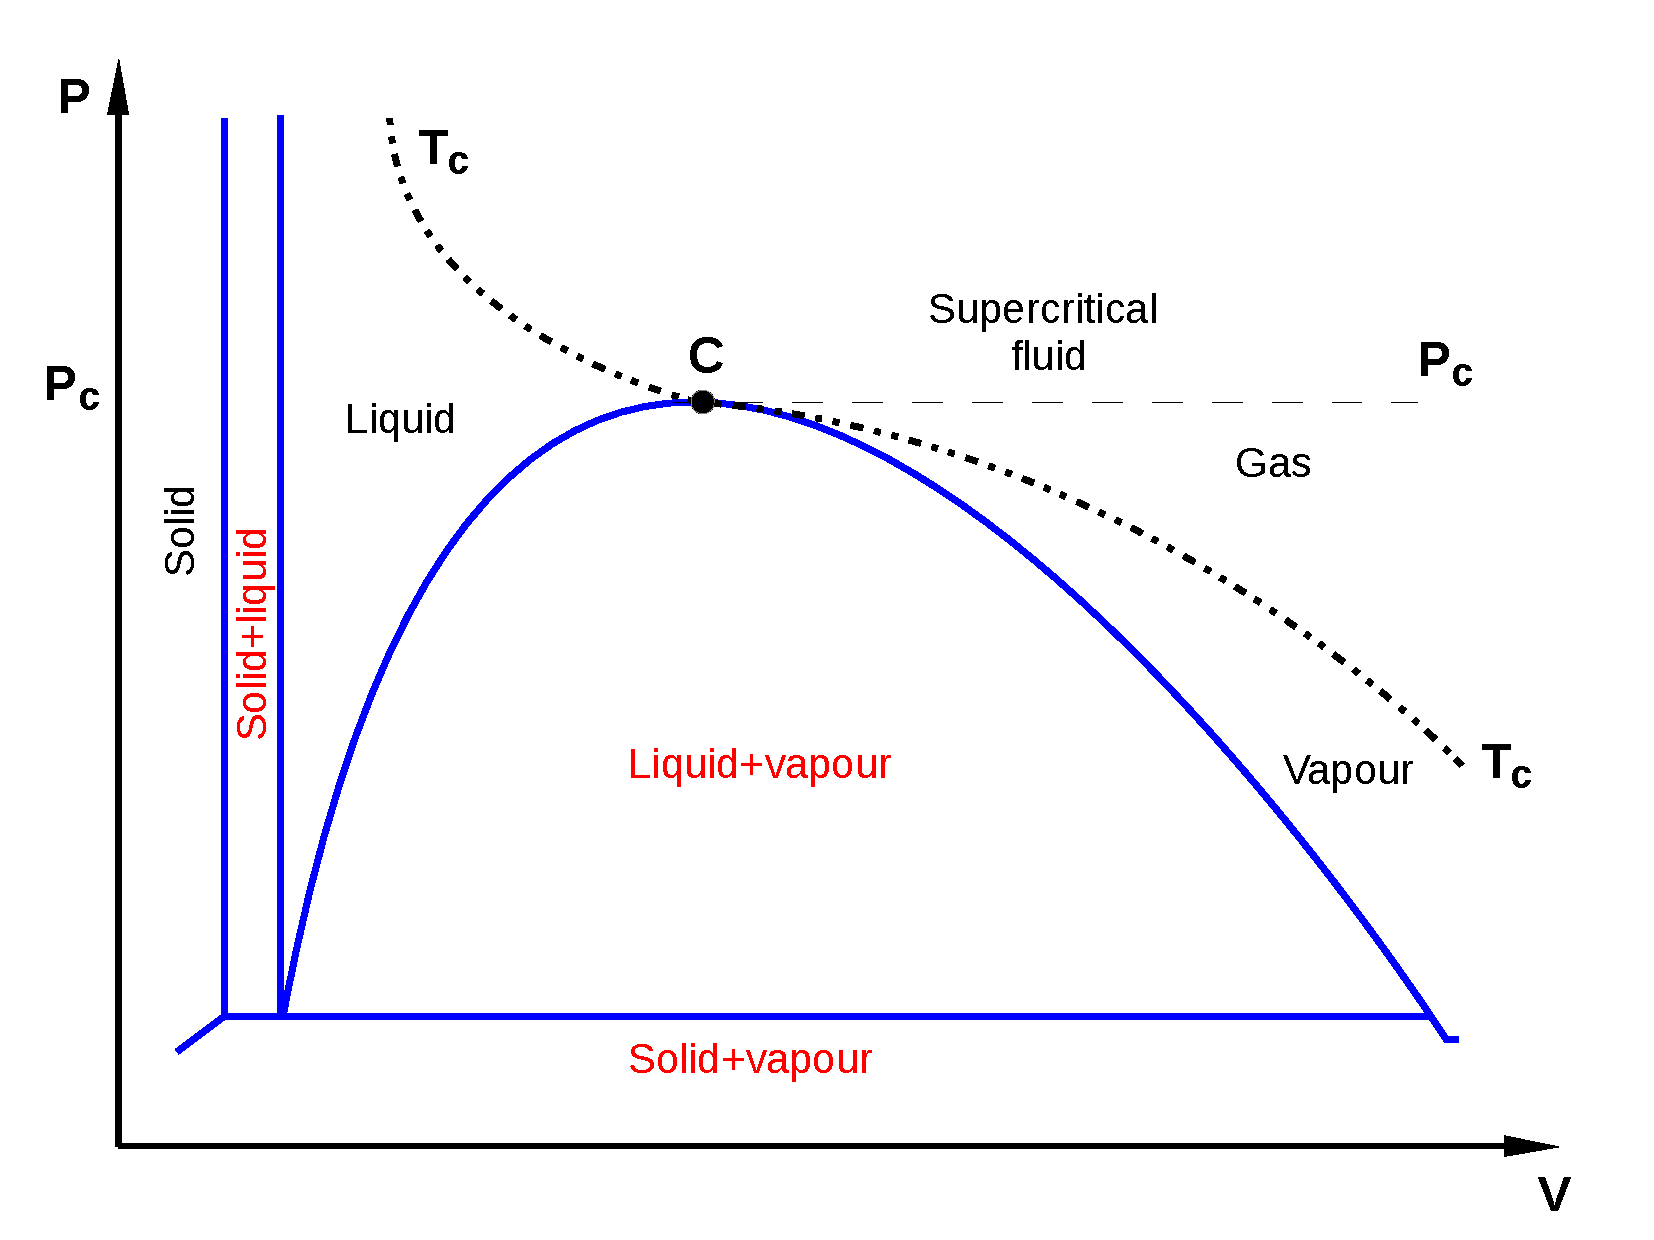
\includegraphics[width=.5\columnwidth,clip]{./Figs/PV_Diagram1}
                          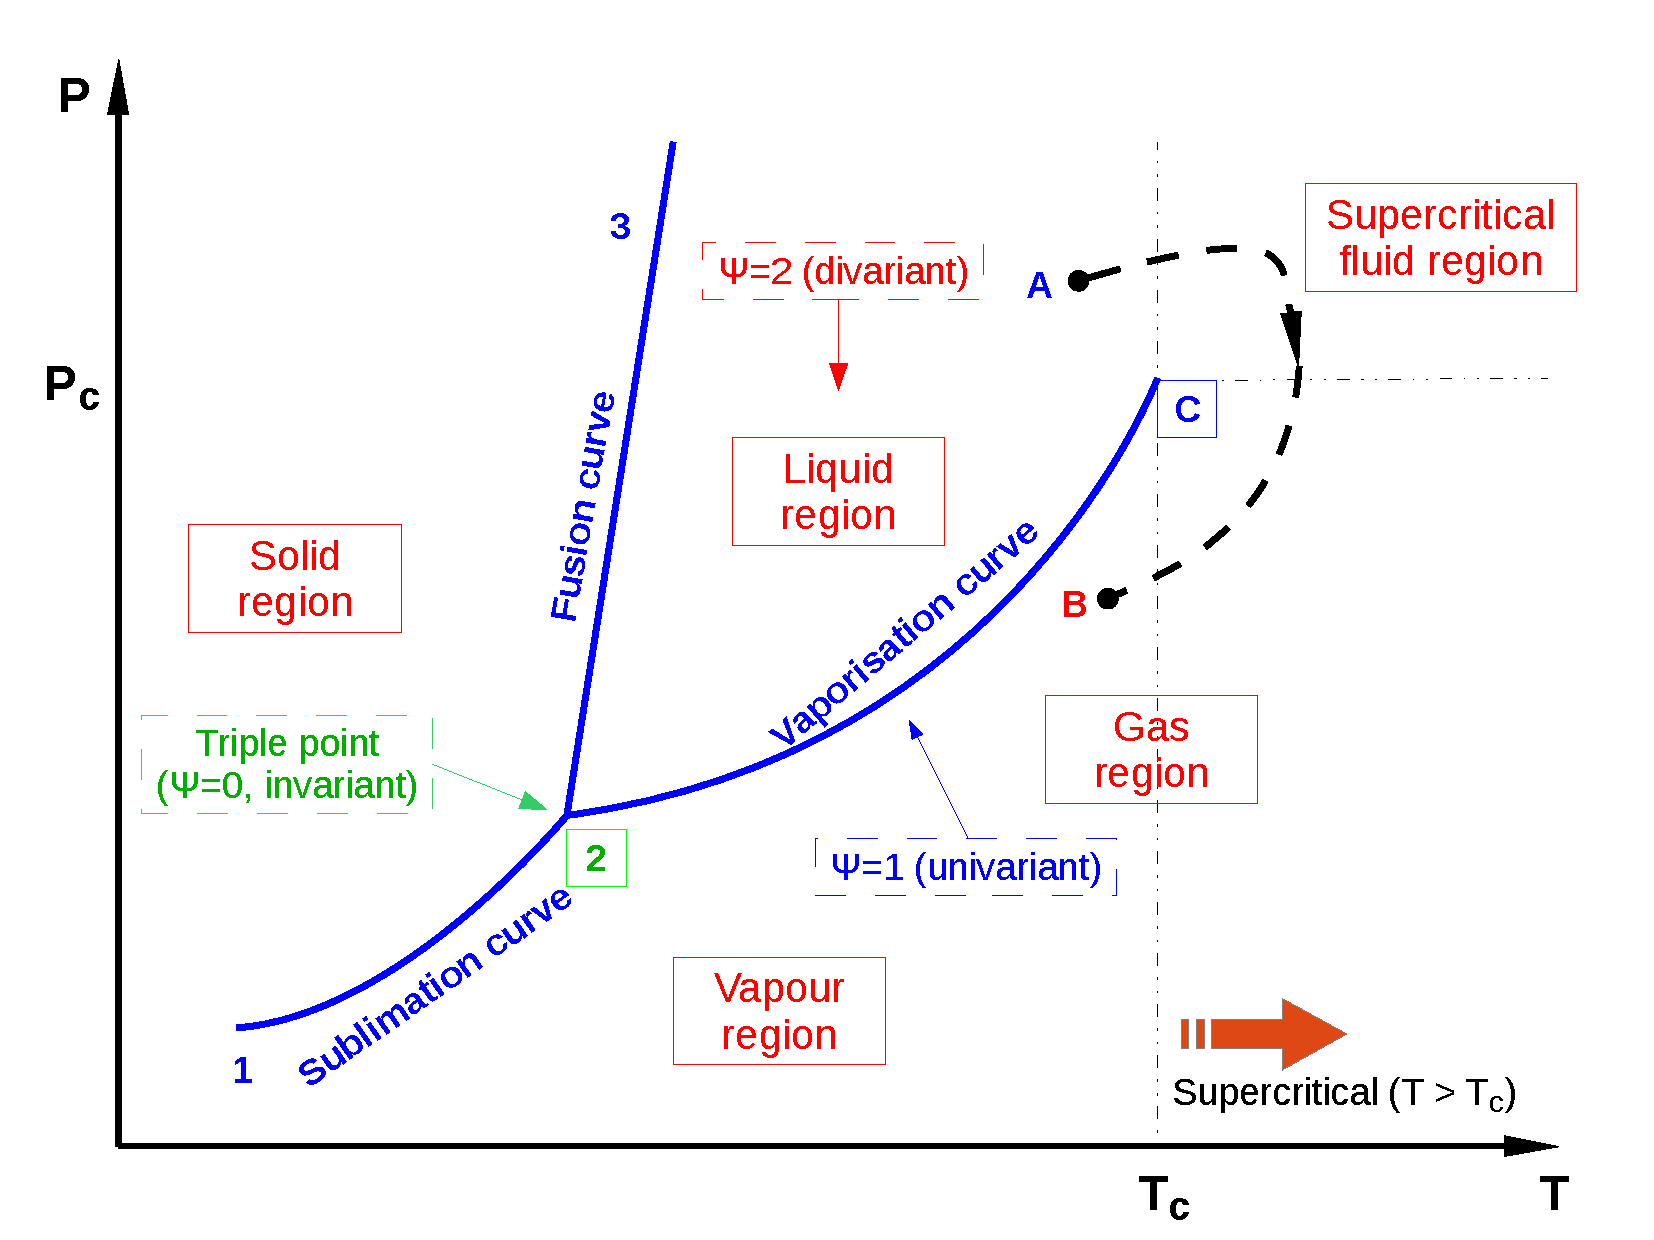
\includegraphics[width=.5\columnwidth,clip]{./Figs/PT_Diagram}}
                    \vspace{-.1cm}
                    \hbox{\hspace{4cm}(a)\hspace{8cm}(b)}}
              \caption{ (a) $PV$ and (b) $PT$ diagrams for a pure substance. Dotted line in (a) represents the isotherm at T=T$_{c}$.}\label{Chapter:VolumetricPropertiesPureSubstances:Fig:PV-PT_Diagrams}
           \end{figure}


           In vapour-liquid equilibrium (VLE) systems there are two main saturation lines: {\it saturated liquid line} (left-hand side of $C$ in Fig.~\ref{Chapter:VolumetricPropertiesPureSubstances:Fig:PV-PT_Diagrams}a)  and {\it saturated vapour line} (rhs of $C$) that represent the initial transition from a single phase system to a two or three phases system. 
%

$PT$ diagrams (Fig.~\ref{Chapter:VolumetricPropertiesPureSubstances:Fig:PV-PT_Diagrams}b) are representations of Fig.~\ref{Chapter:VolumetricPropertiesPureSubstances:Fig:PVT_Surfaces}a, where phases are defined by surfaces (\ie areas) with continuous lines representing phases transitions (\ie in equilibrium). The {\it triple point} is coordinate in which all three phases (S, L and V) coexist in equilibrium.

A fluid in the compressed liquid state is often called {\it sub-cooled fluid} (central region of Fig.~\ref{Chapter:VolumetricPropertiesPureSubstances:Fig:PV-PT_Diagrams}b), while a gas at a pressure lower than its saturation vapour pressure for a given temperature is said to be at {\it superheated state}.


%%% SECTION
%%%
\section{Gibbs Phase Rule}\label{Chapter:VolumetricPropertiesPureSubstances:Section:GibbsPhaseRule}\index{Gibbs phase rule}
\begin{subequations}
  Let's consider a non-reactive system in equilibrium within $\mathcal{P}$ phases  (\ie $L$, $V$ and/or $S$) containing $\mathcal{N}$ independent chemical species.  The number of degrees of freedom for the system (\ie the number of intensive variables that may vary independently) may be expressed as,
  \begin{shaded}
    \begin{center}
      Degrees of freedom = (Number of intensive variables) – (Number of independent equations),
    \end{center}
  \end{shaded}
  \noindent where
  \begin{itemize}
    \item Number of intensive variables: $T$, $P$ and $\left(\mathcal{N}-1\right)$ species mole fractions for each of the $\mathcal{P}$ phases;
    \item Number of independent equations: $\left(\mathcal{P}-1\right)\mathcal{N}$.
  \end{itemize}
  


  
The complete description of the state of a system must include the value of an extensive
variable of each phase (e.g., the volume, mass, or amount) in order to specify how much of
the phase is present. For an equilibrium system of P phases with a total of 3 independent
variables, we may choose the remaining 3 P variables to be intensive. The number of these
intensive independent variables is called the number of degrees of freedom or variance,
  
  The Gibbs phase rule is a relation that determines the number of independent variables that must be specified to establish the intensive state of any system at equilibrium ,
                \begin{equation}
                    \Psi = 2 + \mathcal{C} - \mathcal{P} -\mathcal{R},\label{Mod02_GibbsPhaseRuleReactive}
                \end{equation}
                where $\Psi$, $\mathcal{C}$, $\mathcal{P}$ and $\mathcal{R}$ are the number of degrees of freedom of the thermodynamic system, number of chemical components, number of co-existing phases and number of independent reactions, respectively. For non-reactive systems\footnote{The Gibbs phase rule will be revisited again in Module~\ref{Section:06} -- Chemical Reaction Equilibrium.}, this relation becomes,
                \begin{equation}
                    \Psi = 2 + \mathcal{C} - \mathcal{P}.\label{Mod02_GibbsPhaseRule}
                \end{equation}
                The degrees of freedom ($\Psi$, \ie number of intensive properties such as temperature and pressure) determines the number of variables that must be specified to fix all other remaining phase rule variables. For example, for a pure liquid component, the phase rule yields two degrees of freedom, \ie if temperature and pressure are specified, all other intensive properties (\eg enthalpy, entropy etc) are uniquely determined. However, if the same liquid component is in equilibrium with its vapour phase (\eg water and steam) there is {\it only} one degree of freedom. This means that either pressure or temperature may be specified to fix all other intensive properties of the system. At the triple point (\eg water, steam and ice), the number of degrees of freedom is {\it zero}, \ie any change from such state (\eg for water-steam-ice at $\sim$ 273.15 K and 0.0061 bar) causes at least one of the phases to vanish.
\end{subequations}

%%% SECTION
\section{PVT Behaviour of Pure Substances}\label{Chapter:VolumetricPropertiesPureSubstances:PVTBehaviour}
  
   \begin{enumerate}[i)]
%
%
%
        
%
        \item The ideal gas {\it equation of state} (EOS),
                \begin{equation}
                   P V = R T,\label{Mod02_IdealEOS}
                \end{equation}
                where $V$ is the molar volume. This is a relationship between the macroscopic intensive properties, and is based in two main assumptions with respect to the microscopic behaviour of molecules:
            \begin{enumerate}[(a)]
                \item Molecules have no extension in space (\ie zero volume), and;
                \item Molecules \underline{do not interact with each other}.
            \end{enumerate}
            The second assumption is particularly important as it considers that atoms and molecules either do not interact or do not have electric charge or have an infinite distance between them (\ie low density conditions).
%
        \item However, these assumptions are rarely met in real conditions (both in the environment and in industry) and several mathematical relations have been developed to better represent the PVT behaviour of real fluids:
            \begin{enumerate}[a)]
%
                \item The PVT behaviour of real pure fluids can be expressed as functional $f(P,V,T) = 0$. However, from the Gibbs phase rule for a single phase pure component the number of degrees of freedom is equal to 2. Therefore, we can write this function in its simplest way (or EOS), $V=V(T,P)$, or in differential form,
                   \begin{displaymath}
                      dV = \left(\frc{\partial V}{\partial T}\right)_{P}dT + \left(\frc{\partial V}{\partial P}\right)_{T}dP
                   \end{displaymath}
                   defining the {\it coefficient of thermal expansion} (or {\it volume expansivity coefficient}), $\beta$, and the {\it coefficient of isothermal compressibility}, $\kappa$ as,
                   \begin{equation}
                      \beta \equiv \frc{1}{V}\left(\frc{\partial V}{\partial T}\right)_{P}\;\;\;\text{ and }\;\;\;\kappa \equiv -\frc{1}{V}\left(\frc{\partial V}{\partial P}\right)_{T},\label{Mod02_Compressibilityexpansivity}
                   \end{equation}
                   respectively, leading to
                   \begin{equation}
                       \frc{dV}{V} = \beta dT - \kappa dP.\label{Mod02_Compressibilityexpansivity2}
                   \end{equation}
%
                \item The {\it Virial EOS} is a relation that can be derived from statistical mechanics, and is represented by power series in terms of $\frac{1}{V}$ with two alternate forms:
                   \begin{eqnarray}
                       \frc{P V}{R T} &=& 1 + \frc{B}{V} + \frc{C}{V^{2}} + \cdots \text{ or} \label{Mod02_Virial1}\\
                       \frc{P V}{R T} &=& 1 + B^{\prime}P + C^{\prime}P^{2} + \cdots,\label{Mod02_Virial2} 
                   \end{eqnarray}
                   where $B$ and $C$ are the second and third virial coefficients and,
                   \begin{displaymath}
                      B = \frc{B^{\prime}}{R T}\;\;\;\text{ and }\;\;\; C^{\prime}=\frc{C-B^{2}}{\left(R T\right)^{2}}.
                   \end{displaymath}
                   Second and third terms of Eqns.~\ref{Mod02_Virial1} and~\ref{Mod02_Virial2} are \blue{corrections of the non-ideal behaviour of a gas}. Virial coefficients are strongly dependent on the temperature (\ie $B=B(T)$, $C=C(T)$, $D=D(T)$ etc) and the more the number of coefficients (\ie the more terms in the power series -- Eqns.~\ref{Mod02_Virial1} and~\ref{Mod02_Virial2}) the better is the predictions of the gas molar volume. The second virial coefficient is readily found for a large number of fluids in any chemical engineering handbook (and several textbooks), however the third and further coefficients are more difficult to obtain/calculate. Therefore the Virial EOS is often used for moderate deviations from the ideal gas behaviour through the truncated forms of Eqns.~\ref{Mod02_Virial1} and~\ref{Mod02_Virial2}
                   \begin{eqnarray}
                      \frc{P V}{R T} &=& 1 + \frc{B}{V} \;\;\;\;\text{ or } \label{Mod02_Virial1b}\\
                      Z &=& 1 + \frc{B P}{R T} = 1 + \frc{B P_{c}}{R T_{c}}\frc{P_{r}}{T_{r}},\label{Mod02_Virial1c}
                   \end{eqnarray}
                   where,
                   \begin{equation}
                      T_{r} = \frc{T}{T_{c}}\;\;\;\;\text{ and }\;\;\;\; P_{r} = \frc{P}{P_{c}}\label{Mod02_ReducedT-P},
                   \end{equation}
                   are {\it reduced temperature and pressure}, respectively. $Z = \frac{P V}{R T}$ is the \underline{compressibility factor} and can be defined as the ratio of the molar volume of a gas to the molar volume of an ideal gas at the same temperature and pressure conditions -- for an ideal gas, $Z=1$. 

                   A number of {\it generalised relations} have been developed to calculate the {\it second virial coefficients}, \eg
                   \begin{displaymath}
                      \frc{B P_{c}}{R T_{c}} = B^{0} + \omega B^{1},
                   \end{displaymath}
                   with terms $B^{0}$ and $B^{1}$ defined by,
                   \begin{displaymath}
                      B^{0} = 0.083 - \frc{0.422}{T_{r}^{1.6}}\;\;\text{ and }\;\; B^{1} = 0.139 - \frc{0.172}{T_{r}^{4.2}}.
                   \end{displaymath}
                   $\omega$ is a parameter known as \underline{acentric factor} that measures the non-sphericity of molecules,
                   \begin{displaymath}
                      \omega \equiv -1 - \log\limits_{10}{\left(P_{r}^{\text{sat}}\right)_{T_{r}=0.7}},
                   \end{displaymath}
                   where $\left(P_{r}^{\text{sat}}\right)_{T_{r}=0.7}$ is the reduced saturation vapour pressure obtained at reduced temperature of 0.7. Tabulated acentric factor for a number of chemical species can be found in any thermodynamic textbook.
%
                \item The truncated form of the {\it Virial EOS} can be used to represent PVT behaviour of gases with reasonable accuracy at relatively low pressures. At moderate and high pressures, predicted volumetric properties deviate from expected and alternative EOS formulations have been developed. \underline{Cubic EOS} are widely used in \blue{flow and process simulators} to represent PVT behaviour of fluids, and were developed as a cubic function of the molar volume (or the compressibility factor, $Z$). Cubic equations of state can result in (reasonable) accurate prediction of both gas and liquid (saturated) molar volumes and are relatively easy to implement. Since the development of the first cubic EOS in the 19$^{\text{th}}$ century, several EOS have been proposed and used by industry. Four of the most important cubic EOS are listed below:
                   \begin{enumerate}[c.1)]
%
                      \item The \underline{van der Walls} (vdW) EOS was originally developed in 1873 and has the form,
                          \begin{equation}
                             P = \frc{R T}{V-b} - \frc{a}{V^{2}},\label{Mod02_vdWEOS}
                          \end{equation}
                          where $a$ is called the {\it attraction parameter} and $b$ is the {\it repulsive parameter} (or {\it effective molecular volume} or {\it co-volume}), 
                          \begin{displaymath}
                              a = \frc{27}{64}\frc{R^{2}T_{c}^{2}}{P_{c}},\;\;\; b = \frc{1}{8}\frc{R T_{c}}{P_{c}},
                          \end{displaymath}
                          and they take into account interactions between molecules. Although this EOS is able to predict volumetric properties of gasses better than the ideal EOS, it is still very inaccurate for liquids and for fluids at high pressure.  Redlich-Kwong and Soave-Redlich-Kwong EOS were formulated in the 40's and 70's and became increasingly popular in the oil $\&$ gas and petrochemical sectors. 
%
                      \item Redlich-Kwong (RK EOS):
                           \begin{equation}
                               P = \frc{R T}{V-b} - \frc{a}{V\sqrt{T}\left(V+b\right)},\label{Mod02_RKEOS}
                           \end{equation}
                           with,
                          \begin{displaymath}
                              a = \frc{0.42748 R^{2}T_{c}^{2}}{P_{c}},\; \text{ and }\;\;\; b = \frc{0.08664 R T_{c} }{P_{c}}.
                          \end{displaymath}
%
                      \item Soave-Redlich-Kwong (SRK EOS):
                           \begin{equation}
                               P = \frc{R T}{V-b} - \frc{a\alpha}{V\left(V+b\right)},\label{Mod02_SRKEOS}
                           \end{equation}
                           with,
                          \begin{eqnarray}
                              &&a = \frc{0.427 R^{2}T_{c}^{2}}{P_{c}},\;\;\;b = \frc{0.08664 R T_{c} }{P_{c}} \nonumber \\
                              &&\text{and }\;\;\; \alpha = \left[1 + \left( 0.48508 + 1.55171\omega - 0.15613\omega^{2}\right)\left(1-\sqrt{T_{r}}\right)\right]^{2}\nonumber
                          \end{eqnarray}                          
%
                      \item Peng-Robinson (PR EOS): it is by far the most used EOS used in simulators and is able to predict molar volume with good accuracy,
                           \begin{equation}
                               P = \frc{R T}{V-b} - \frc{a\alpha}{V\left(V+b\right)+b\left(V-b\right)},\label{Mod02_PREOS}
                           \end{equation}
                           with,
                          \begin{eqnarray}
                              && a = \frc{0.45724 R^{2}T_{c}^{2}}{P_{c}},\;\;\;b = \frc{0.07780 R T_{c} }{P_{c}},\;\;\alpha = \left[1 + \kappa\left(1-\sqrt{T_{r}}\right)\right]^{2}  \nonumber \\
                              &&\text{ and }\; \kappa = 0.37464 + 1.54226\omega - 0.26992\omega^{2} \nonumber
                          \end{eqnarray}                
%
                   \end{enumerate}
                   These EOS can be generalised and manipulated to appear as a cubic function of the compressibility factor, $Z$,
                   \begin{equation}
                      Z^{3} + k_{1} Z^{2} +k_{2} Z + k_{3} = 0,\label{Mod02_GeneralEOS}
                   \end{equation}
                   where
                   \begin{eqnarray}
                     && A = \frc{aP}{\left(RT\right)^{2}},\;\; B = \frc{bP}{RT},\;\; k_{1} = -1 -B + uB, \nonumber \\
                     && k_{2} = A + w B^{2} - uB -uB^{2}\;\;\text{ and }\;\; k_{3} = - AB -w B^{2} -w B^{3}.\nonumber
                   \end{eqnarray}

\begin{table}[h]
  \begin{center}
  \begin{tabular}{ c | c c c c c }
    \hline
      {\bf EOS} & {\bf $u$} & {\bf $w$} & {\bf k$_{1}$} & {\bf k$_{2}$} & {\bf k$_{3}$} \\
    \hline
        {\bf vdW} &    0    &    0    & -1-B       &     A         & -AB         \\
        {\bf RK}  &    1    &    0    & -1         &  A-B-B$^{2}$   & -AB         \\
        {\bf SRK} &    1    &    0    & -1         &  A-B-B$^{2}$   & -AB         \\
        {\bf PR}  &    2    &   -1    & -1+B       & A-2B-3B$^{2}$  & -AB+B$^{2}$+B$^{3}$ \\
    \hline
  \end{tabular}
  \caption{Values for $u$, $w$ and k$_{i}$ for vdW, RK, SRK and PR EOS --  Eqn.~\ref{Mod02_GeneralEOS}.}\label{Mod02:Table1}
  \end{center}
\end{table}
                   Coefficients for these expressions are listed in Table~\ref{Mod02:Table1}. Equation~\ref{Mod02_GeneralEOS} has three roots ($Z_{1}$, $Z_{2}$ and $Z_{3}$), the largest \underline{real positive root} represents the {\it vapour phase}, $Z_{\text{vap}}$, whereas the \underline{smallest real positive root} represents the {\it liquid phase}, $Z_{\text{liq}}$, the intermediate root has no physical meaning. The relevant roots for this cubic polynomial can be obtained from the following relations:
                   \begin{eqnarray}
                       Z_{\text{vap}} &=& 1 + \beta - q\beta \frc{Z_{\text{vap}} - \beta} {\left(Z_{\text{vap}}+\varepsilon\beta\right)\left(Z_{\text{vap}} +\sigma\beta\right)},\label{Mod02_Zvap} \\
                       Z_{\text{liq}} &=& 1 + \beta + \left(Z_{\text{liq}} + \epsilon\beta\right)\left(Z_{\text{liq}}+\sigma\beta\right)\left(\frc{1+\beta-Z_{\text{liq}}}{q\beta}\right)\label{Mod02_Zliq}
                   \end{eqnarray}
                   with 
                   \begin{displaymath}
                      \beta=\Omega\frc{P_{r}}{T_{r}},\;\;\; \text{ and }\;\;\; q=\frc{\Psi\alpha}{\Omega T_{r}}.
                   \end{displaymath}
                   Parameters for these expressions are listed in Table~\ref{Mod02:Table2} with
                   \begin{eqnarray}
                         \alpha_{\text{SRK}} &=& \left[ 1 + \left( 0.480 + 1.574 \omega - 0.176\omega^{2}\right)\left(1-\sqrt{T_{r}}\right)\right]^{2}, \nonumber \\
                         \alpha_{\text{PR}} &=& \left[ 1 + \left( 0.37464 + 1.54226 \omega - 0.26992\omega^{2}\right)\left(1-\sqrt{T_{r}}\right)\right]^{2}. \nonumber
                   \end{eqnarray}
                   Equations~\ref{Mod02_Zvap} and ~\ref{Mod02_Zliq} can be numerically solved either by a {\it calculator} or applying any method described in Appendix \red{E.2} (see Example~\ref{Mod02Ex01}).

\begin{table}[h]
    \begin{center}
       \begin{tabular}{| l | c c c c c| }
       \hline
          {\bf EOS}  & {\bf $\alpha$} & {\bf $\sigma$}  & {\bf $\varepsilon$} & {\bf $\Omega$} & {\bf $\Psi$ } \\
       \hline
            vdW      & 1              & 0               & 0                  & 1/8            & 27/64          \\
            RK       & T$_{r}^{-1/2}$  & 1                & 0                  & 0.08664       & 0.42748        \\
           SRK       &$\alpha_{\text{SRK}}$& 1            & 0                   & 0.08664       & 0.42748        \\
            PR       &$\alpha_{\text{PR}}$& 1+$\sqrt{2}$   & 1-$\sqrt{2}$        & 0.07780        & 0.45724  \\
       \hline
       \end{tabular}
  \caption{Parameters for Eqns.~\ref{Mod02_Zvap}-~\ref{Mod02_Zliq}.}\label{Mod02:Table2}
  \end{center}
\end{table}

                  

%
            \end{enumerate}
% 
   \end{enumerate}

\clearpage

%%% SUBSECTION
\subsection{Examples}

\begin{enumerate}[1)]
%%%
%%% EXAMPLE 
%%%
\item\label{Mod02Ex01} For gaseous methane at 298K and 2 MPa, compute the molar volume $\left(\text{in cm}^{3}.\text{mol}^{-1}\right)$ using the SRK EOS. Given $T_{c}=$ 190.7 K, $P_{c}=$ 46.41 bar and $\omega=$ 0.011.

% SOLUTION
        \noindent{\bf Solution:} We can calculate the molar volume of a real gas using the relation $PV=ZRT$, where the compressibility factor for the gaseous fluid can be obtained from Eqn.~\ref{Mod02_Zvap},
           \begin{displaymath}
                Z_{\text{vap}} = 1 + \beta - q\beta \frc{Z_{\text{vap}} - \beta} {\left(Z_{\text{vap}}+\varepsilon\beta\right)\left(Z_{\text{vap}} +\sigma\beta\right)},
           \end{displaymath}
           where 
           \begin{eqnarray}
               && T_{r}=\frc{T}{T_{c}} = 1.5627,\;\;P_{r}=\frc{P}{P_{c}}=0.4309,\;\;\omega=0.011,\;\;\Omega = 0.08664, \nonumber \\
               && \Psi = 0.42748,\;\; \sigma=1.0,\;\;\epsilon=0.0,\;\;\beta=\Omega\frc{P_{r}}{T_{r}}=2.3890\times 10^{-2},\nonumber \\
               && \alpha_{\text{SRK}} = 0.7667\;\;\text{ and }\;\; q = \frc{\Psi\alpha_{\text{SRK}}}{\Omega T_{r}} = 2.4207, \nonumber 
           \end{eqnarray}

           There are three ways to solve this non-linear equation, all of them involve iterative methods for root-finder
           \begin{enumerate}[a)]
%
              \item Using a calculator, leading to $Z_{\text{vap}} = $ 0.9670. 
%
              \item {\bf Substitution method:} In this method we rewrite the $Z_{\text{vap}}$ equation as,
                 \begin{displaymath}
                     Z_{\text{vap}}^{(i+1)} = 1 + \beta - q\beta \frc{Z_{\text{vap}}^{(i)} - \beta} {\left(Z_{\text{vap}}^{(i)}+\varepsilon\beta\right)\left(Z_{\text{vap}}^{(i)} +\sigma\beta\right)},
                 \end{displaymath}
                 where $i(=1, 2, \cdots n_{\text{max}})$ is an index for the number of iterations and $n_{\text{max}}$ is the total number of iterations. Taking the ideal gas condition as the initial guess in this iterative method, \ie $Z_{\text{vap}}^{(1)}=1$, 
                 \begin{eqnarray}
                    i=1 &\Rightarrow& Z_{\text{vap}}^{(2)} = 1 + \beta - q\beta \frc{Z_{\text{vap}}^{(1)} - \beta} {\left(Z_{\text{vap}}^{(1)}+\varepsilon\beta\right)\left(Z_{\text{vap}}^{(1)} +\sigma\beta\right)} = 0.96876 \nonumber \\
                    i=2 &\Rightarrow& Z_{\text{vap}}^{(3)} = 1 + \beta - q\beta \frc{Z_{\text{vap}}^{(2)} - \beta} {\left(Z_{\text{vap}}^{(2)}+\varepsilon\beta\right)\left(Z_{\text{vap}}^{(2)} +\sigma\beta\right)} = 0.96707 \nonumber \\
                    i=3 &\Rightarrow& Z_{\text{vap}}^{(4)} = 1 + \beta - q\beta \frc{Z_{\text{vap}}^{(3)} - \beta} {\left(Z_{\text{vap}}^{(3)}+\varepsilon\beta\right)\left(Z_{\text{vap}}^{(3)} +\sigma\beta\right)} = 0.96697 \nonumber \\
                    i=4 &\Rightarrow& Z_{\text{vap}}^{(5)} = 1 + \beta - q\beta \frc{Z_{\text{vap}}^{(4)} - \beta} {\left(Z_{\text{vap}}^{(4)}+\varepsilon\beta\right)\left(Z_{\text{vap}}^{(4)} +\sigma\beta\right)} = 0.96696 \nonumber \\
                    \vdots && \vdots \nonumber
                 \end{eqnarray}
                 these iterations can continue 'till either $i=n_{\text{max}}$ (\ie we reached the maximum number of iterations) or solution has converged (\ie there is no significant change in the solution after k$^{\text{th}}$ iteration). We can create a {\it stoppage criteria} to acess if the solution converged,
                 \begin{displaymath}
                      \mathcal{E} = \frc{\| Z_{\text{vap}}^{(i+1)} - Z_{\text{vap}}^{(i)}\|}{Z_{\text{vap}}^{(i)}}.
                 \end{displaymath}
                 If $\mathcal{E}$ is smaller than a prescribed tolerance, than we say that the method converged, otherwise we should continue our iterations. Assuming that $\mathcal{E} \leq 1.0\times 10^{-4}$,
                 \begin{center}
                     \begin{tabular}{c c c c}
                        \hline
                            $\mathbf{i}$  &  $\mathbf{Z_\text{vap}^{(i)}}$  & $\mathbf{Z_\text{vap}^{(i+1)}}$  & $\mathbf{\mathcal{E}}$ \\  
                               1         &           1.0                 &  0.96876                      &  3.12$\times$10$^{-2}$ \\
                               2         &       0.96876                 &  0.96707                      &  1.74$\times$10$^{-3}$ \\
                               3         &       0.96707                 &  0.96697                      &  1.03$\times$10$^{-4}$ \\
                               4         &       0.96697                 &  0.96696                      &  1.03$\times$10$^{-5}$ \\  
                        \hline
                     \end{tabular}
                 \end{center}
                 Thus after the forth iteration the solution converged to $Z_{\text{vap}}^{(4)} = 0.96696 \sim 0.9670$.
%
              \item {\bf Newton-Raphson Method:} This iterative method (see Appendix E.2) is based on dividing the domain in infinitesimal segments and smoothly `walking towards the solution'. It can be generalised as,
                  \begin{displaymath}
                     x^{(i+1)} = x^{(i)} - \frc{F\left(x^{(i)}\right)}{F^{\prime}\left(x^{(i)}\right)},
                  \end{displaymath}  
                  where $F^{\prime}\left(x^{(i)}\right) = \frc{d F\left(x^{(i)}\right)}{dx}$, \ie the first derivative of the function. In our case, the first step is to manipulate our $Z_{\text{vap}}$ equation as,
                  \begin{displaymath}
                     F\left(Z_{\text{vap}}\right) = Z_{\text{vap}} - 1 - \beta + q\beta \frc{Z_{\text{vap}} - \beta} {\left(Z_{\text{vap}}+\varepsilon\beta\right)\left(Z_{\text{vap}} +\sigma\beta\right)},
                  \end{displaymath}
                  and the Newton-Raphson Method becomes,
                  \begin{displaymath}
                     Z_{\text{vap}}^{(i+1)} = Z_{\text{vap}}^{(i)} - \frc{F\left(Z_{\text{vap}}^{(i)}\right)}{F^{\prime}\left(Z_{\text{vap}}^{(i)}\right)}.
                  \end{displaymath}
                  The next step is to obtain the derivative of the function $F\left(Z_{\text{vap}}\right)$ with respect to $Z_{\text{vap}}$, \ie (for $\epsilon=0$)
                  \begin{eqnarray}
                     F^{\prime}\left(Z_{\text{vap}}\right) &=& \frc{d F^{\prime}\left(Z_{\text{vap}}\right)}{d Z_{\text{vap}}} = \frc{d}{dZ_{\text{vap}}} \left[Z_{\text{vap}} - 1 - \beta + q\beta \frc{Z_{\text{vap}}-\beta}{Z_{\text{vap}}\left(Z_{\text{vap}}+\sigma\beta\right)}\right]\nonumber \\
                                                       &=& 1 - \frc{q\beta}{\left(Z_{\text{vap}}+\sigma\beta\right)^{2}} + \frc{q\beta^{2}\left(2Z_{\text{vap}}+\sigma\beta\right)}{\left[Z_{\text{vap}}\left(Z_{\text{vap}}+\sigma\beta\right)\right]^{2}}. \nonumber
                  \end{eqnarray}
                  This leads to,
                  \begin{eqnarray}
                     Z_{\text{vap}}^{(i+1)} &=& Z_{\text{vap}}^{(i)} - \frc{F\left(Z_{\text{vap}}^{(i)}\right)}{F^{\prime}\left(Z_{\text{vap}}^{(i)}\right)} \nonumber \\
                     &=& Z_{\text{vap}}^{(i)} - \frc{Z_{\text{vap}}^{(i)} - 1 - \beta + q\beta \frc{Z_{\text{vap}}^{(i)} - \beta} {Z_{\text{vap}}^{(i)}\left(Z_{\text{vap}}^{(i)} +\sigma\beta\right)}}{1 - \frc{q\beta}{\left(Z_{\text{vap}}^{(i)}+\sigma\beta\right)^{2}} + \frc{q\beta^{2}\left(2Z_{\text{vap}}^{(i)}+\sigma\beta\right)}{\left[Z_{\text{vap}}^{(i)}\left(Z_{\text{vap}}^{(i)}+\sigma\beta\right)\right]^{2}}}. \nonumber
                  \end{eqnarray}
                  Using ideal gas as initial guess, \ie $Z_{\text{vap}}^{(1)}=1$ and $\mathcal{E} \leq 1.0\times 10^{-4}$,
                 \begin{center}
                     \begin{tabular}{c c c c}
                        \hline
                            $\mathbf{i}$  &  $\mathbf{Z_\text{vap}^{(i)}}$  & $\mathbf{Z_\text{vap}^{(i+1)}}$  & $\mathbf{\epsilon}$ \\  
                               1         &           1.0                 &  0.96703                      &  3.30$\times$10$^{-2}$ \\
                               2         &       0.96703                 &  0.96697                      &  6.20$\times$10$^{-5}$ \\
                               3         &       0.96697                 &  0.96697                      & $<$ 1$\times$10$^{-5}$ \\ 
                        \hline
                     \end{tabular}
                 \end{center}
                 The solution rapidly converged after the second iteration to $Z_{\text{vap}}^{(2)}=0.96697\sim 0.9670$. 
%
           \end{enumerate}
\medskip

           Now replacing $Z_{\text{vap}} = 0.9670$ in 
           \begin{displaymath}
              V=\frc{Z_{\text{vap}}R T}{P} = 1197.9493 \text{ cm}^{3}.\text{mol}^{-1}\sim 1197.95 \text{ cm}^{3}.\text{mol}^{-1}
           \end{displaymath}
\clearpage
%%%
%%% EXAMPLE 
%%%
\item\label{Mod02Ex02} Calculate the molar volume $\left(\text{in cm}^{3}.\text{mol}^{-1}\right)$ for gaseous butane at 2.5 bar and 298 K using (a) the ideal gas equation, (b) the truncated virial EOS and (c) the PR EOS. Given $T_{c}=$ 425.1 K, $P_{c}=$ 37.96 bar and $\omega=$ 0.20.

% SOLUTION
        \noindent{\bf Solution:} 
           \begin{enumerate}[a)]
%
               \item Assuming that butane behaves as an ideal gas,
                    \begin{displaymath}
                        V^{\text{IG}} = \frc{RT}{P} = 9910.6456 \text{ cm}^{3}.\text{mol}^{-1}
                    \end{displaymath}
%
               \item From Eqn.~\ref{Mod02_Virial1c},
                  \begin{displaymath}
                     Z = \frc{P V}{R T} = 1 + \frc{B P_{c}}{R T_{c}}\frc{P_{r}}{T_{r}},
                  \end{displaymath}
                  manipulating this equation with 
                  \begin{displaymath}
                     \frc{B P_{c}}{R T_{c}} = B^{0} + \omega B^{1},
                  \end{displaymath}
                  leads to
                  \begin{displaymath}
                     V = \frc{R T}{P} + \left(B^{0} + \omega B^{1}\right) \frc{P_{r}R T}{T_{r}P} = \frc{R T}{P} + \left(B^{0} + \omega B^{1}\right)\frc{RT_{c}}{P_{c}},
                  \end{displaymath}
                  where $P_{r}=\frac{P}{P_{c}}$ and $T_{r}=\frac{T}{T_{c}}$. Calculating $B^{0}$ and $B^{1}$ from
                  \begin{displaymath}
                     B^{0} = 0.083 - \frc{0.422}{T_{r}^{1.6}} = -0.6620\;\;\text{ and }\;\; B^{1} = 0.139 - \frc{0.172}{T_{r}^{4.2}}=-0.6257.
                  \end{displaymath}
                  Thus $V^{\text{virial}} = 9430.6465$ cm$^{3}$.mol$^{-1}$.
%
               \item Now, in order to calculate the molar volume using the PR EOS, we first need to calculate the compressibility factor $Z_{\text{vap}}$, Eqn.~\ref{Mod02_Zvap},
                  \begin{displaymath}
                     Z_{\text{vap}} = 1 + \beta - q\beta \frc{Z - \beta} {\left(Z+\varepsilon\beta\right)\left(Z+\sigma\beta\right)},
                  \end{displaymath}
                  with
                  \begin{eqnarray}
                     && T_{r}=\frc{T}{T_{c}} = 0.7010,\;\;P_{r}=\frc{P}{P_{c}}=6.5859\times 10^{-2},\;\;\omega=0.20,\;\;\Omega = 0.07880, \nonumber \\
                     && \Psi = 0.45724,\;\; \sigma=1+\sqrt{2},\;\;\epsilon=1-\sqrt{2},\;\;\beta=\Omega\frc{P_{r}}{T_{r}}=7.3281\times 10^{-4},\nonumber \\
                     && \alpha_{\text{PR}} = 1.2308\;\;\text{ and }\;\; q = \frc{\Psi\alpha_{\text{PR}}}{\Omega T_{r}} = 102.9246, \nonumber 
                  \end{eqnarray}
                  Solving numerically leads to $Z_{\text{vap}}=0.9188$ and $V=\frc{Z_{\text{vap}}RT}{P} = 9105.9012$ cm$^{3}$.mol$^{-1}$.
%
           \end{enumerate}
\clearpage
%%%
%%% EXAMPLE 
%%%
   \item\label{Mod02Ex03} Derive the relations for coefficient of thermal expansion and the isothermal compressibility coefficient for
              \begin{enumerate}[(a)]
                  \item Ideal gas EOS;
                  \item $V=\frc{a}{RT}+\frc{bT}{PR}$ 
              \end{enumerate}

% SOLUTION
        \noindent{\bf Solution:} Here we need to obtain expressions for 
           \begin{eqnarray}
                && \beta = \frc{1}{V}\left(\frc{\partial V}{\partial T}\right)_{P} \nonumber \\
                && \kappa = -\frc{1}{V}\left(\frc{\partial V}{\partial P}\right)_{T} \nonumber
           \end{eqnarray}
           for 
           \begin{enumerate}[a)]
%
               \item Ideal gas EOS, $V=\frc{R T}{P}$,
                    \begin{displaymath}
                       \beta =\frc{P}{R T}\frc{R}{P} = \frc{1}{T},
                    \end{displaymath}
                    and 
                    \begin{displaymath}
                       \kappa = -\frc{P}{R T}\left(-\frc{R T}{P^{2}}\right) = \frc{1}{P}
                    \end{displaymath}
%
               \item $V=\frc{a}{RT}+\frc{bT}{PR}$: Solving the partial differentials,
                    \begin{displaymath}
                       \left(\frc{\partial V}{\partial T}\right)_{P} = \frc{b}{PR}-\frc{a}{RT^{2}}\;\;\text{ and }\;\; \left(\frc{\partial V}{\partial P}\right)_{T} = -\frc{bT}{P^{2}R},
                    \end{displaymath}
                    thus
                    \begin{eqnarray}
                       && \beta =\frc{1}{\frc{a}{RT}+\frc{bT}{PR}}\left(\frc{b}{PR}-\frc{a}{RT^{2}}\right) = \frc{\frc{bT^{2}-aP}{PRT^{2}}}{\frc{aP+bT^{2}}{PRT}} = \frc{bT^{2}-aP}{T\left(aP+bT^{2}\right)}
 \nonumber \\
                       && \kappa = -\frc{1}{\frc{a}{RT}+\frc{bT}{PR}} \left(-\frc{bT}{P^{2}R}\right) = \frc{bT^{2}}{P\left(aP+bT^{2}\right)} \nonumber
                    \end{eqnarray}
                    
%
           \end{enumerate}
%     
\end{enumerate}
